

Decision trees have long been recognized as one of the most interpretable machine learning models due to their transparent hierarchical structure and human-readable decision rules \cite{10.1145/2783258.2788613, wang2022timbertrek, lin2022generalizedscalableoptimalsparse, ustun2019learningoptimizedriskscores}. The effective visualization of decision trees for interpretability is an active area of research, with significant implications for eXplainable Artificial Intelligence and human-AI interaction. The challenge extends beyond simply displaying the tree structure to creating interfaces that support comprehensive understanding, analysis, and interaction with both the model and the underlying data.

The literature on decision tree visualization spans 
from traditional node-link diagrams to sophisticated interactive systems. Hans-Jorg Schulz \cite{schulz2011treevis} provides a comprehensive survey identifying over 180 tree visualization techniques, categorizing them by dimensionality (2D, 3D, or hybrid), edge representation (explicit, implicit, or hybrid), and node alignment (radial, axis-parallel, or free). This taxonomic foundation reveals the breadth of approaches available, yet also highlights the fragmented nature of the field, where many techniques have been developed independently without systematic comparison.

Recent advances in the field emphasize the critical importance of integrating visualization with interaction and algorithmic support. Van den Elzen et al. \cite{elzen2011baobabview} demonstrate that effective decision tree systems require tight coupling between these three components, enabling domain experts to incorporate their knowledge into both tree construction and analysis processes. Their BaobabView system, shown in Figure \ref{fig:baobab_interface}, exemplifies this integration by supporting interactive growing, pruning, optimization, and analysis of decision trees through coordinated visual interfaces.

% Source: BaobabView Interactive Construction and Analysis of Decision Trees, Page: Figure 3
\begin{figure}[!htb]
    \centering
    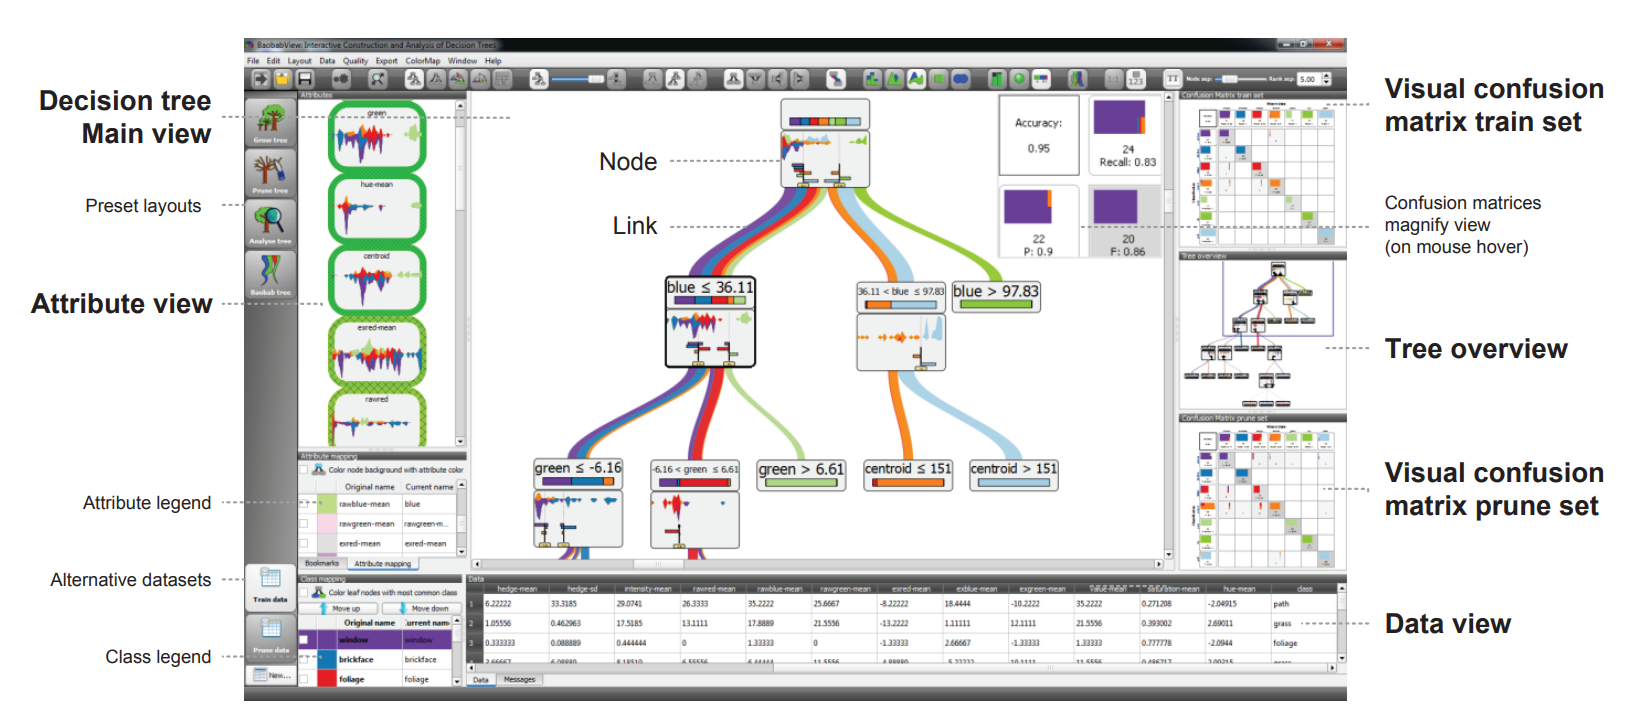
\includegraphics[width=\linewidth]{images/baobabView UI.png}
    \caption{Interface of the interactive decision tree construction software BaobabView with the proposed decision tree visualization. Based on adapted node-link diagram, nodes contain important decision tree components while links are visualized as a stream of items flowing between nodes. The interface integrates decision tree main view, attribute view, visual confusion matrices, tree overview, and data view for comprehensive analysis.}
    \label{fig:baobab_interface}
\end{figure}

The application domains for decision tree visualization are diverse, with particular emphasis on high-stakes decision-making contexts. In medical applications, Jakub Mrva et al. \cite{mrva2019decision} explore 3D visualization techniques that not only display tree structure but also reveal correlations between attributes and decision impacts, as demonstrated in Figure \ref{fig:3d_medical_trees}. 

% Source: Decision Support in Medical Data Using 3D Decision Tree Visualisation, Multiple pages
\begin{figure}
  \centering

  \begin{subfigure}[c]{0.95\textwidth}
    \centering
    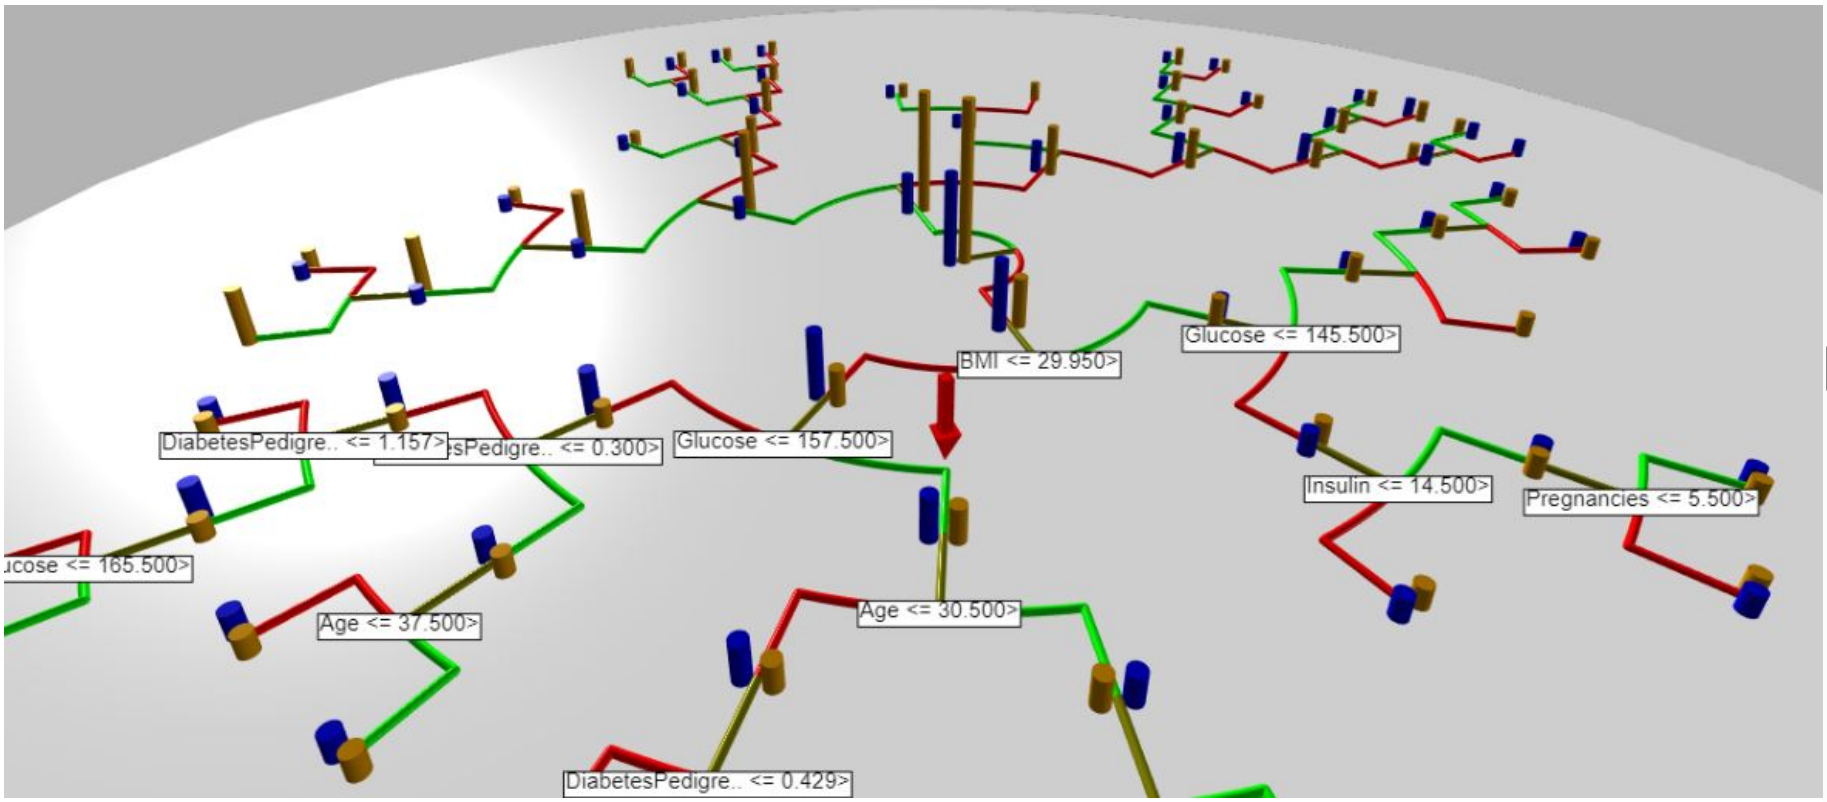
\includegraphics[width=\linewidth]{images/3D Decision Tree1.png}
    \caption{Visualization displaying the overall structure of the trained decision tree on diabetes dataset. Focused node is marked by the arrow.}
    \label{fig:top}
  \end{subfigure}

  \vspace{6pt} 

  \begin{subfigure}[c]{0.48\textwidth}
    \centering
    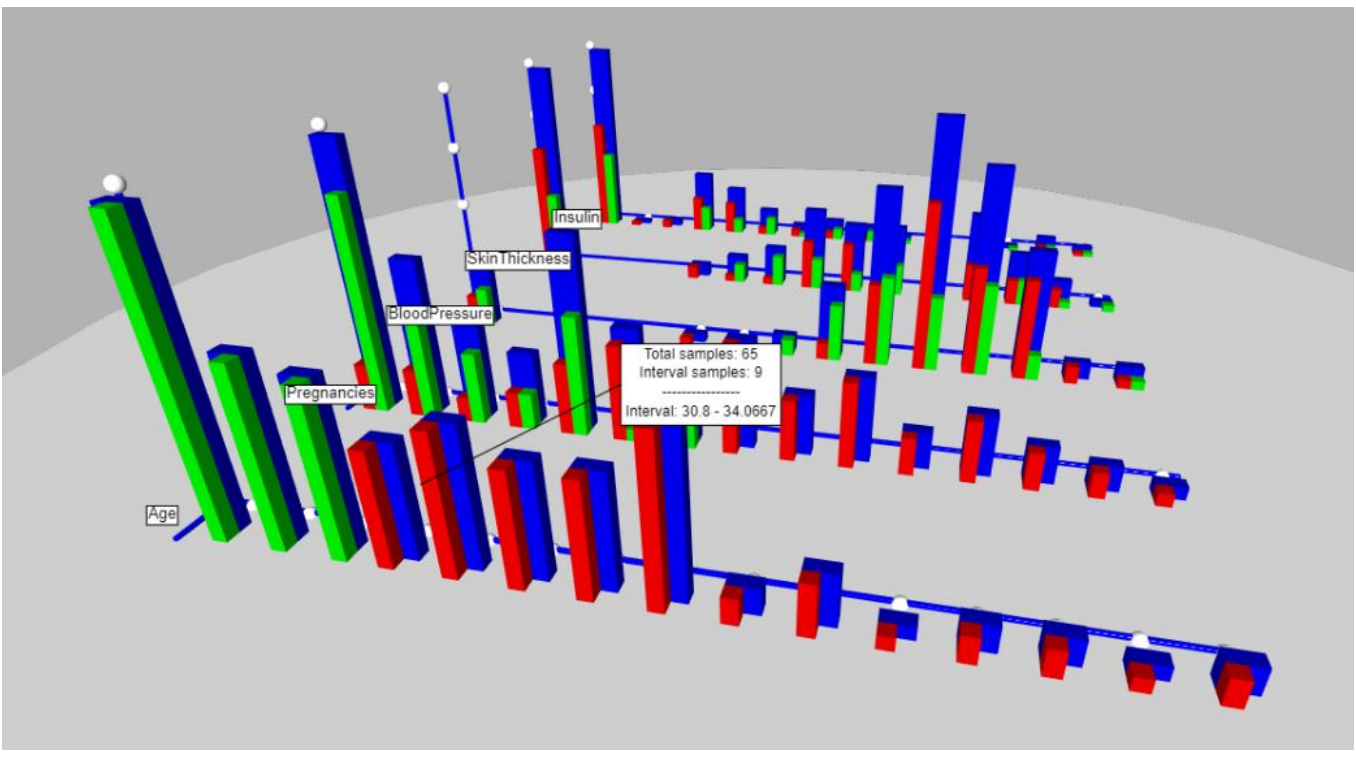
\includegraphics[width=\linewidth]{images/3D Decision Tree2.png} 
    \caption{A focused view on one decision tree node. The first set of histograms
displays attribute used in the split. Following sets display correlated attributes.}
    \label{fig:bottom-left}
  \end{subfigure}
  \hfill
  \begin{subfigure}[c]{0.48\textwidth}
    \centering
    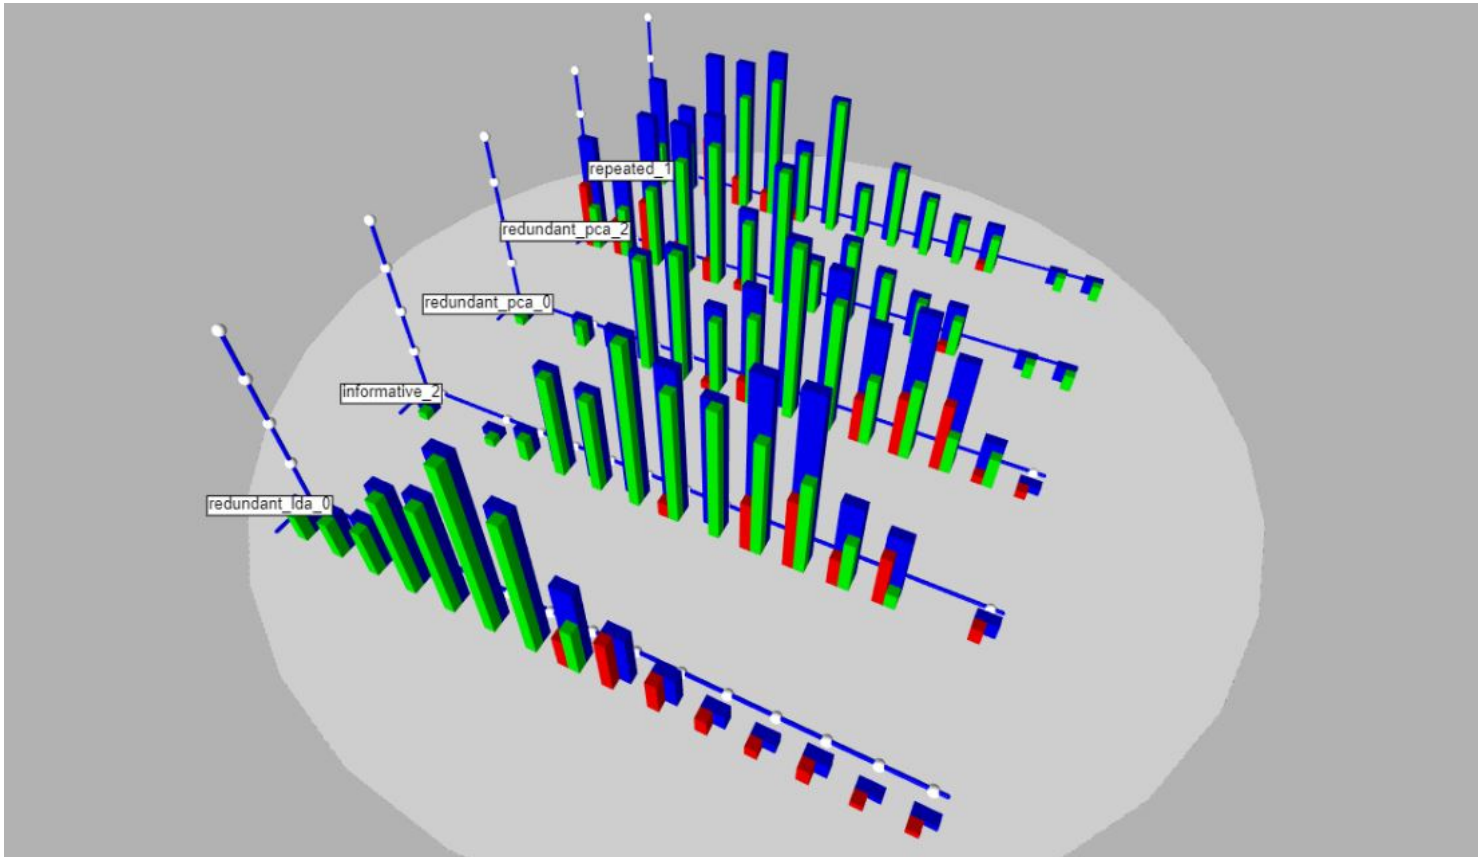
\includegraphics[width=\linewidth]{images/3D Decision Tree3.png}
    \caption{A detailed view on a decision rule in a single node and histograms for
other attribute values of both data subsets divided by the node. Histograms in
decreasing dissimilarity order highlight most important differences. }
    \label{fig:bottom-right}
  \end{subfigure}

    \caption{3D decision tree visualization for medical data using circular plane layout. Nodes are positioned based on depth from the root, with 3D bar charts and histograms showing class distributions and feature relationships. This approach emphasizes visualization of attribute correlations beyond the primary splitting criterion.}
    \label{fig:3d_medical_trees}
\end{figure}

A significant trend in recent literature is the handling of high-dimensional data and complex model spaces. Szücs et al. \cite{szucs2018decision} deal with the challenge of visualizing decision boundaries in high-dimensional feature spaces through projection strategies, while Wang et al. \cite{wang2022timbertrek} address the problem of model selection from large sets of equally-performing trees through their innovative Rashomon set visualization shown in Figure \ref{fig:timbertrek_system}. These works highlight the evolving complexity of decision tree applications and the corresponding need for more sophisticated visualization approaches.

% Source: TimberTrek Exploring and Curating Sparse Decision Trees with Interactive Visualization, Page: Figure 1  
\begin{figure}[ht!]
    \centering
    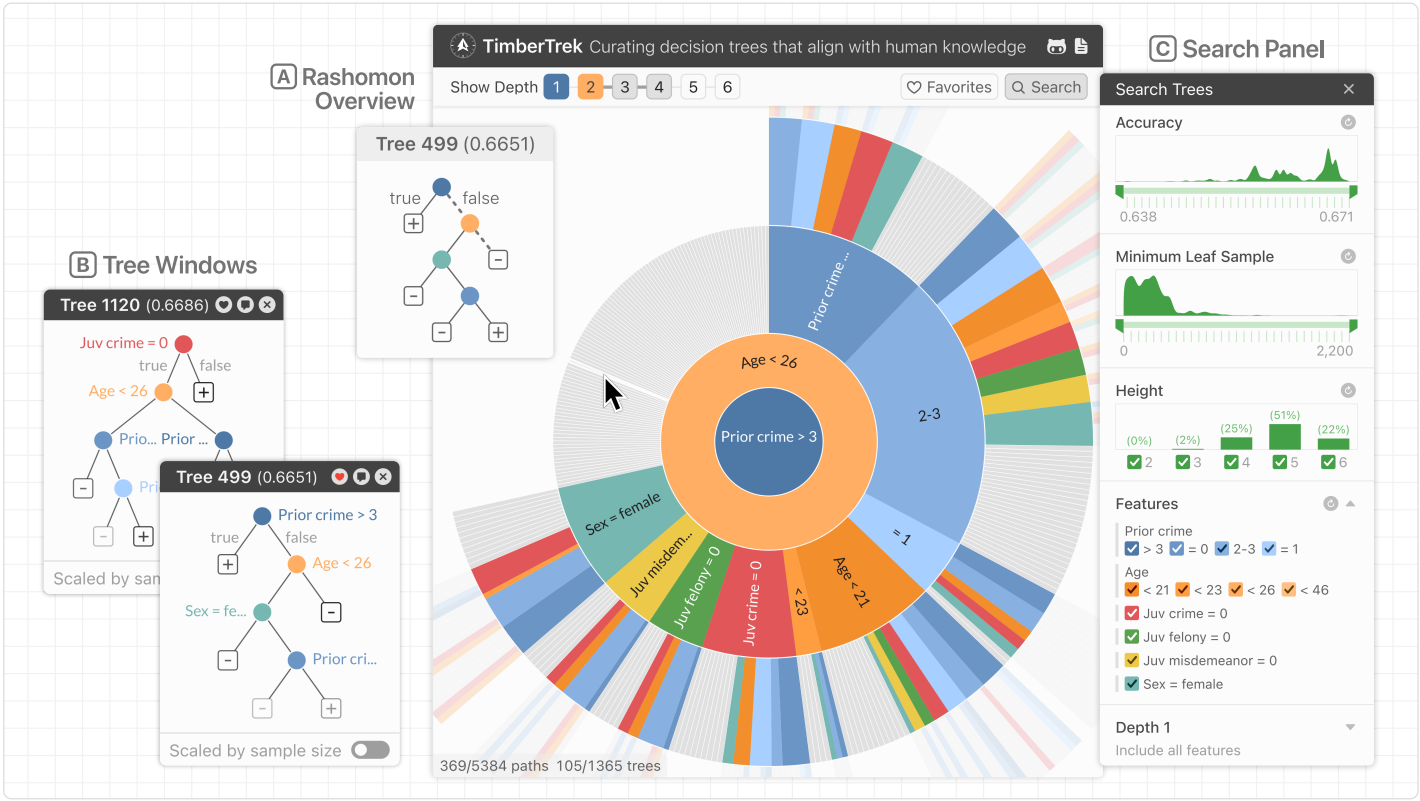
\includegraphics[width=0.95\linewidth]{images/TIMBERTREK .png}
    \caption{TIMBERTREK empowers domain experts and data scientists to easily explore thousands of well-performing decision trees so
they can find and collect those trees that best reflect their knowledge and values. Consider the task of predicting whether a criminal
is likely to commit a crime in the next two years. (A) The Rashomon Overview visually summarizes all well-performing decision trees
by organizing them based on their decision paths, enabling users to seamlessly transition across different model subsets and explore
trees with similar prediction patterns. (B) Clicking a tree opens a repositionable Tree Window showing details of a decision tree:
multiple windows allow users to compare several model candidates’ prediction patterns. (C) The Search Panel provides filtering tools,
enabling users to quickly identify decision trees with desired properties, such as accuracy, robustness, simplicity, and used features.}
    \label{fig:timbertrek_system}
\end{figure}

Interactive capabilities have emerged as a central theme across multiple studies. Kovalerchuk et al. \cite{kovalerchuk2019interactive} demonstrate how interactive threshold modification and dynamic tree construction can enhance model interpretability, while practical tools like dtreeviz \cite{parr2019dtreeviz} focus on providing immediate visual feedback for model validation and debugging. The emphasis on interactivity reflects a broader shift from static visualizations toward dynamic exploration tools that support iterative analysis and refinement.

Despite this rich literature, several gaps remain in current approaches. Most existing visualizations treat the tree structure and the underlying data as separate entities, requiring users to mentally connect model decisions with data distributions. Furthermore, there is limited exploration of how spatial neighborhood analysis plot can be integrated with rule-based interfaces to provide spatial context for
instance-level interpretations. 

\subsubsection{Analysis of Existing Literature and Visualization Techniques}

The literature reveals a diverse ecosystem of decision tree visualization techniques and tools, which can be categorized based on their visual representation approach, interaction paradigm, and target use case. Streeb et al. \cite{Streeb2021TaskBasedVI} provide one of the most comprehensive analyses of this topic, surveying over 150 publications and categorizing them across 16 distinct tasks, 10 possible visual designs, 16 visual designs of further components, and 16 quality measures.
The general results of the evaluation can be observed in Tables \ref{tab:taskStreeb2021TaskBasedVI}, \ref{tab:measureStreeb2021TaskBasedVI} and \ref{tab:VisualDesignsOfTreesANDFurtherComponentsStreeb2021TaskBasedVI}, but the consultation of the publication, currently available at the following link \href{https://el-assady.com/publication/2021streebtask/2021streebtask.pdf}{https://el-assady.com/publication/2021streebtask/2021streebtask.pdf}, is recommended to obtain a full picture of the results and of the reference articles.

{
\footnotesize
\begin{longtable}{|l|*{16}{c|}}
\caption{Tasks \cite{Streeb2021TaskBasedVI}}
\label{tab:taskStreeb2021TaskBasedVI}\\
\hline
\textbf{Ref.} & 
\rotatebox{90}{Concept Introduction} &
\rotatebox{90}{Model Building} &
\rotatebox{90}{Evaluation} &
\rotatebox{90}{Understanding} &
\rotatebox{90}{Diagnosis} &
\rotatebox{90}{Refinement} &
\rotatebox{90}{Comparison} &
\rotatebox{90}{Ensemble Building} &
\rotatebox{90}{Provenance} &
\rotatebox{90}{Reporting} &
\rotatebox{90}{Presentation} &
\rotatebox{90}{Application} &
\rotatebox{90}{Assessment} &
\rotatebox{90}{Monitoring} &
\rotatebox{90}{Decision Modeling} &
\rotatebox{90}{Model Approximation} \\
\hline
\textbf{Total: 152} & 36 & 36 & 34 & 46 & 21 & 8 & 43 & 10 & 3 & 5 & 55 & 6 & 10 & 1 & 11 & 6 \\
\hline
\end{longtable}
}

\begin{table}[ht!]
    \centering
    \caption{Cross-tabulation of tasks and quality measures displayed in the 152 publications Streeb et al. \cite{Streeb2021TaskBasedVI} surveyed. Totals count unique publications in each row/column. Clearly, Accuracy is the most prominently displayed measure of quality. However, compared to the size of our sample quality measures are rarely displayed. There is no relationship apparent between tasks and the quality measures displayed.}
    \label{tab:measureStreeb2021TaskBasedVI}
    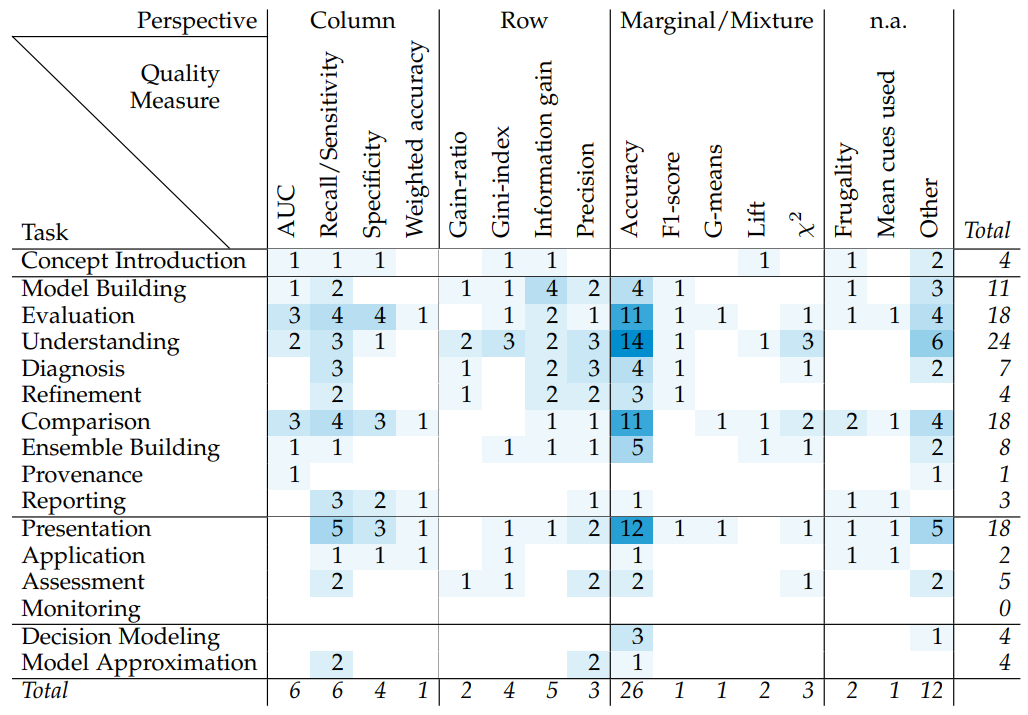
\includegraphics[width=\linewidth]{images/measureStreeb2021TaskBasedVI.png}
\end{table}

\begin{table}
    \centering
    \caption{Cross-tabulation of tasks and quality measures displayed in the 152 publications Streeb et al. \cite{Streeb2021TaskBasedVI} surveyed. Totals count unique publications in each row/column. Clearly, Accuracy is the most prominently displayed measure of quality. However, compared to the size of the analyzed sample, quality measures are rarely displayed. There is no apparent relationship between tasks and the quality measures displayed.}
    \label{tab:VisualDesignsOfTreesANDFurtherComponentsStreeb2021TaskBasedVI}
    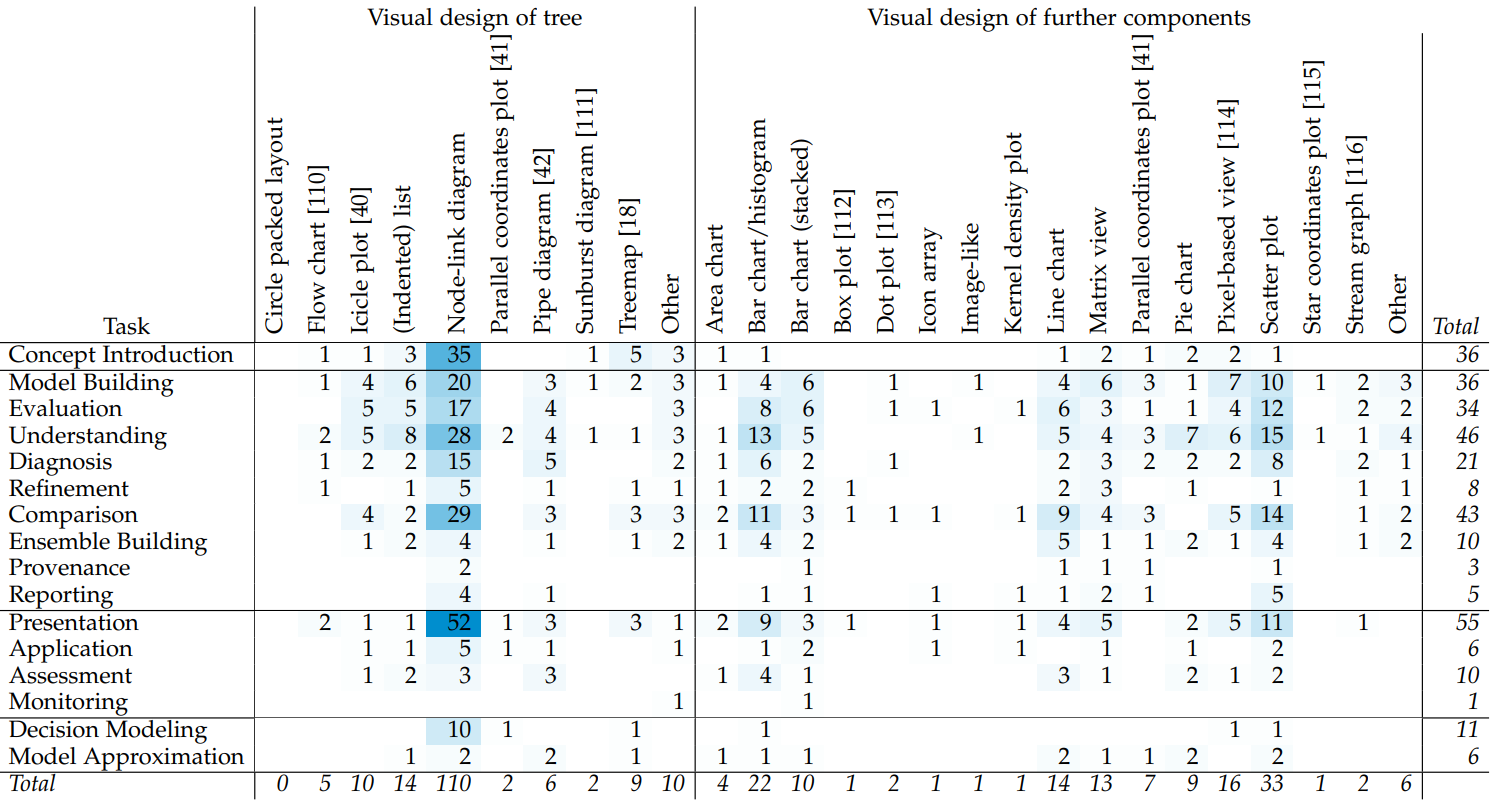
\includegraphics[width=\linewidth]{images/VisualDesignsOfTreesANDFurtherComponentsStreeb2021TaskBasedVI.png}
\end{table}

\paragraph{Traditional Layout Approaches}

The most fundamental category is classical tree layout algorithms. Hans-Jorg Schulz et al. \cite{schulz2011treevis} identify several core approaches including \textbf{node-link diagrams}, which represent the standard hierarchical visualization with explicit connections between parent and child nodes. The evolution of radial tree visualization approaches is particularly well-documented, as shown in Figure \ref{fig:radial_evolution}, which traces the development from natural patterns to interactive systems.

% Source: Treevis.net A Tree Visualization Reference, Page: 14, Figure 1
\begin{figure}[p]
    \centering
    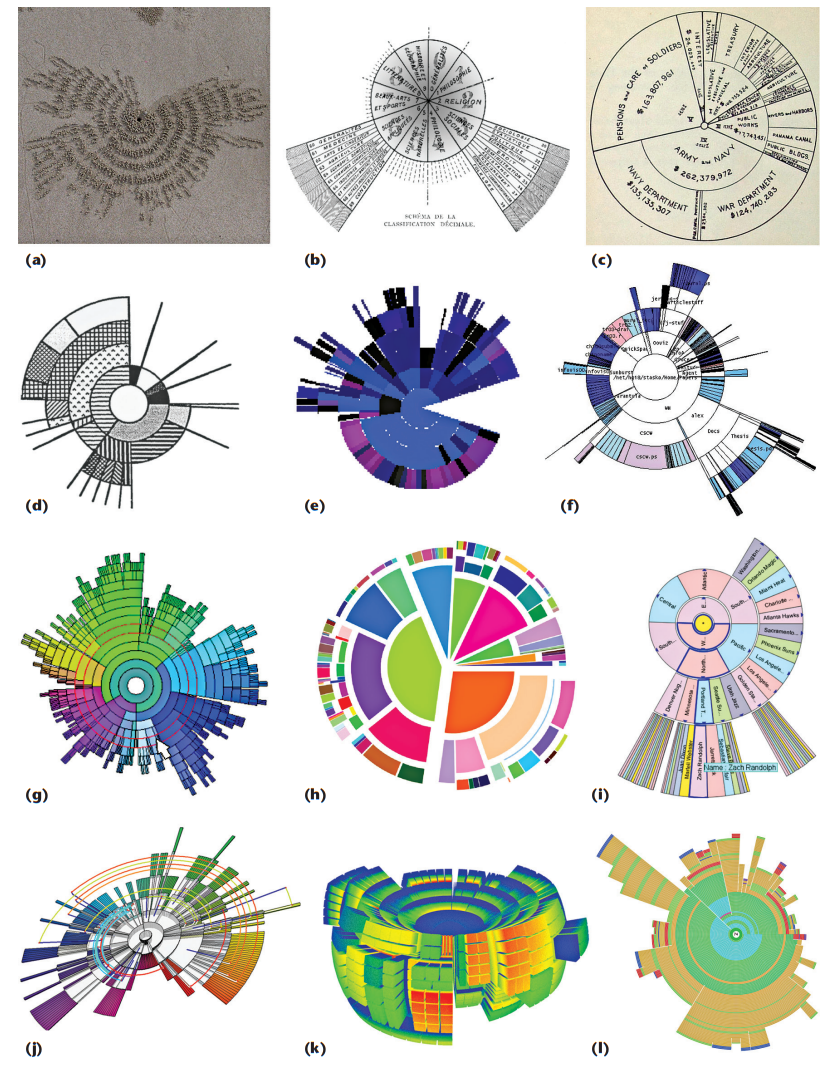
\includegraphics[width=0.85\linewidth]{images/treevis1.png}
    \caption{The evolution of radially stacked tree visualization. (a) Sand bubbler crab pattern (jkr1812 via Flickr).
(b) Universal decimal classification (1905, P. Otlet). (c) Hierarchical sector chart (1921, Am. Soc. Mechanical
Engineers). (d) Spoked polar tree map (1993, B. Johnson). (e) Aggregate tree map (1998, M. Chua). (f) Sunburst
(2000, J. Stasko). (g) Interring (2002, J. Yang et al.). (h) PieTree (2006, R. O’Donnell et al.). (i) FanLens (2008,
X. Lou et al.). (j) Enhanced radial space-filling layout (2009, M. Jia et al.). (k) 3D sunburst wheel (2010, H.-J.
Schulz and S. Hadlak). (l) Trevis calling-context tree ring chart (2010, A. Adamoli and M. Hauswirth). The
fundamental radial design turns out to be much older than most people think.}
    \label{fig:radial_evolution}
\end{figure}

\textbf{Indentation diagrams} provide a text-based alternative where parent-child relationships are conveyed through spatial indentation, though these suffer from poor structural overview for large trees \cite{elzen2011baobabview}. 

\paragraph{Coordinate-Based Visualizations}

A significant body of work explores coordinate system transformations for decision tree representation. Kovalerchuk et al. \cite{kovalerchuk2019interactive} introduce \textbf{General Line Coordinates (GLC)} with two variants: \textbf{Bended Coordinates (BC)} that bend at threshold points, and \textbf{Shifted Paired Coordinates (SPC)} that visualize n-dimensional points as directed graphs in 2D Cartesian coordinates.

\textbf{Parallel coordinates} integration has been explored by multiple researchers \cite{elzen2011baobabview, 10.1007/978-3-540-74205-0_121}, with noting attempts to combine decision trees with parallel coordinate plots, though these suffer from unclear class distribution representation. \textbf{Star coordinate plots} have been employed for interactive tree construction, allowing users to paint areas and assign class labels \cite{elzen2011baobabview, 10.1145/956750.956837, Teoh2003StarClassIV}. The StarClass/PaintingClass system workflow is illustrated in Figure \ref{fig:starclass_workflow}, demonstrating the integration of coordinate-based visualization with interactive model building.

% Source: TaskBased Visual Interactive Modeling Decision Trees and RuleBased Classifiers, Page: Figure 7
\begin{figure}[!htb]
    \centering
    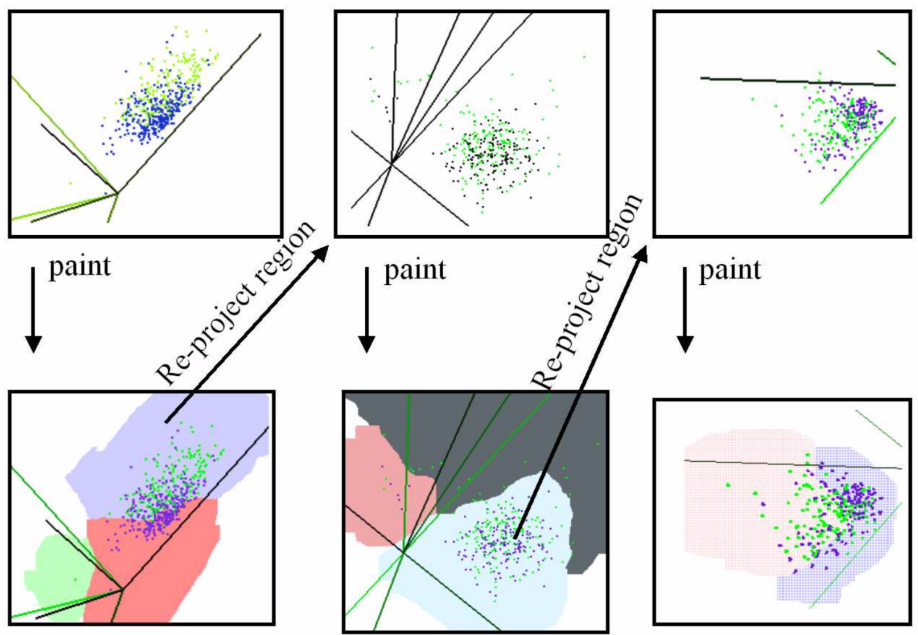
\includegraphics[width=0.9\linewidth]{images/starclass1.png}
    \caption{Workflow and visualization of the StarClass/PaintingClass system \cite{10.1007/978-3-540-74205-0_121, 10.1145/956750.956837}. During model building, analysts use re-projection and painting of regions at different levels of the hierarchy to effectively partition classes in the instance space. The system enables interactive decision boundary creation through direct manipulation of star coordinate projections.}
    \label{fig:starclass_workflow}
\end{figure}

\paragraph{Rule-Based and Matrix Visualizations}

Ming et al. \cite{ming2019rulematrix} pioneered the \textbf{matrix-based visualization} approach, where each row represents a decision rule and each column represents a feature. This technique transforms decision trees into a standardized rule-based knowledge representation, as illustrated in Figure \ref{fig:rulematrix_pipeline}, complemented by \textbf{stream plots} for continuous features and \textbf{stacked bar charts} for categorical features.
One can observe the resulting interface in Figure \ref{fig:rulematrix_interface}.

% Source: TaskBased Visual Interactive Modeling Decision Trees and RuleBased Classifiers, Page: Figure 2
\begin{figure}[!htb]
    \centering
    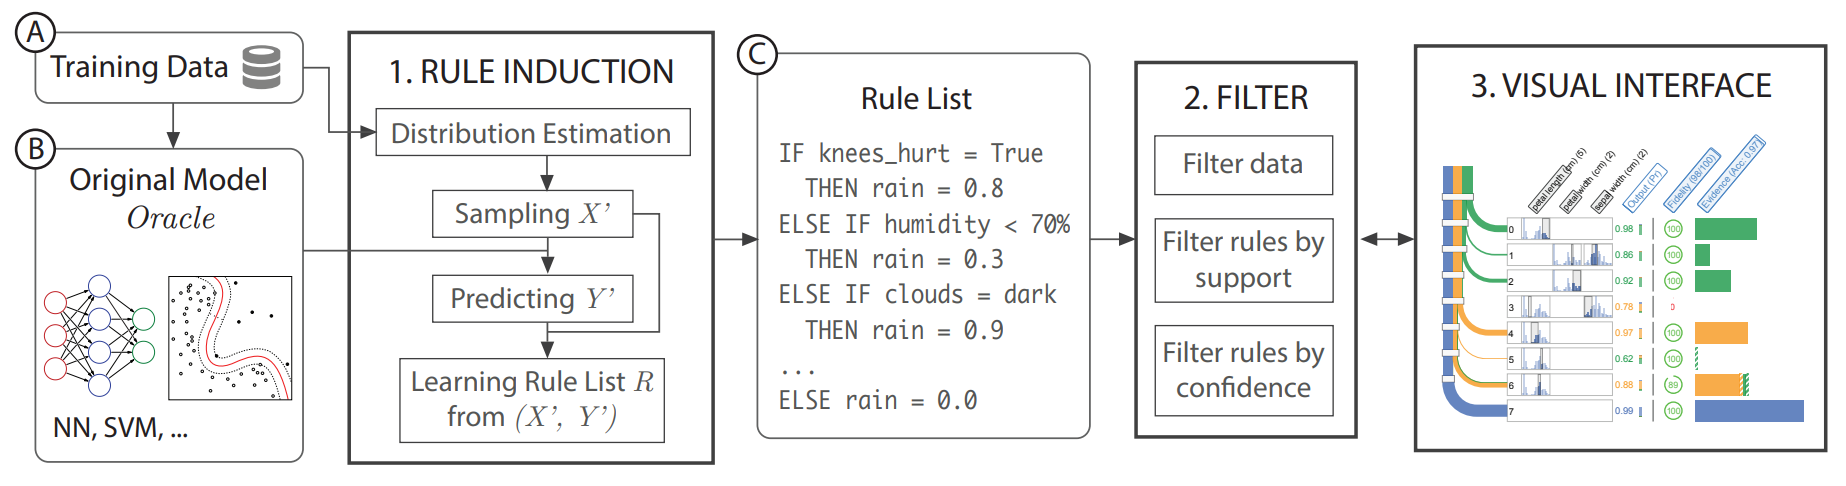
\includegraphics[width=0.9\linewidth]{images/rulematrix1.png}
    \caption{The pipeline for creating a rule-based explanation interface. The rule induction step (1) takes (A) the training data and (B) the model to be
explained as input, and produces (C) a rule list that approximates the original model. Then the rule list is filtered (2) according to user-specified
thresholds of support and confidence. The rule list is visualized as RuleMatrix (3) to help users navigate and analyze the rules.}
    \label{fig:rulematrix_pipeline}
\end{figure}

\begin{figure}[!htb]
    \centering
    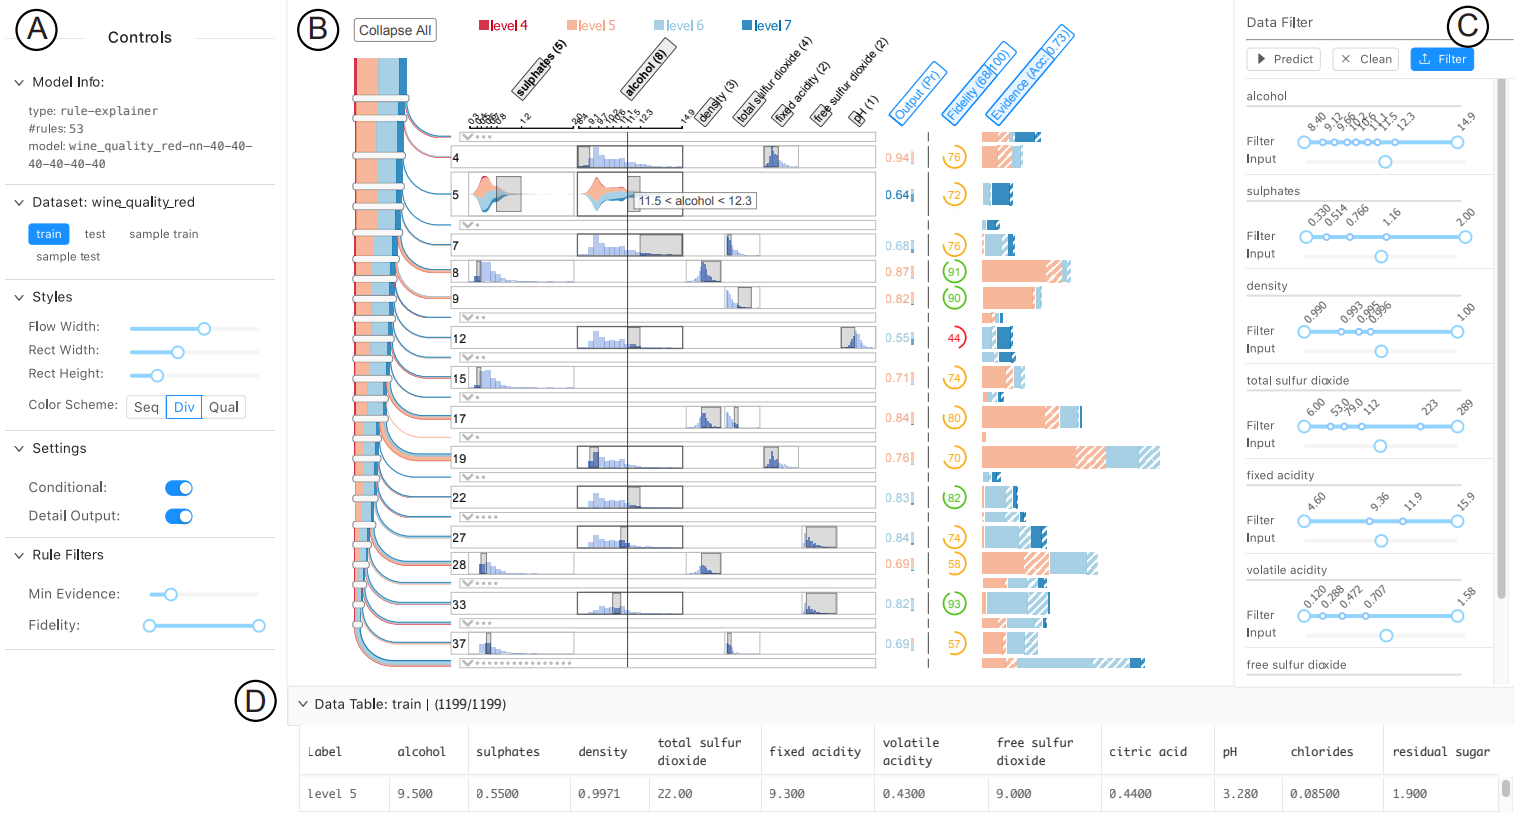
\includegraphics[width=\linewidth]{images/rulematrix2.png}
    \caption{ Understanding the behavior of a trained neural network using the explanatory visual interface of our proposed technique. The
user uses the control panel (A) to specify the detail information to visualize (e.g., level of detail, rule filters). The rule-based explanatory
representation is visualized as a matrix (B), where each row represents a rule, and each column is a feature used in the rules. The
user can also filter the data or use a customized input in the data filter (C) and navigate the filtered dataset in the data table (D).}
    \label{fig:rulematrix_interface}
\end{figure}

\paragraph{3D and Immersive Approaches}

Three-dimensional visualization techniques have been explored for enhanced spatial understanding. Mrva et al. \cite{mrva2019decision} present a \textbf{3D circular plane layout} where nodes are positioned based on depth from the root, with \textbf{3D bar charts} and \textbf{3D histograms} showing class distributions and feature relationships. This approach particularly emphasizes the visualization of attribute correlations beyond the primary splitting criterion, as shown in Figure \ref{fig:3d_medical_trees}.

\paragraph{Interactive and Advanced Visualization Systems}

Several comprehensive systems integrate multiple visualization techniques with interactability. \textbf{BaobabView} \cite{elzen2011baobabview} combines traditional node-link diagrams with integrated confusion matrices, attribute views, and data tables, emphasizing tight integration of visualization, interaction, and algorithmic support. The system's algorithmic support capabilities are detailed in Figure \ref{fig:baobab_algorithmic_support}, which shows how the interface provides visual guidance for split attribute selection.

% Source: TaskBased Visual Interactive Modeling Decision Trees and RuleBased Classifiers, Page: Figure 8
\begin{figure}[!htb]
    \centering
    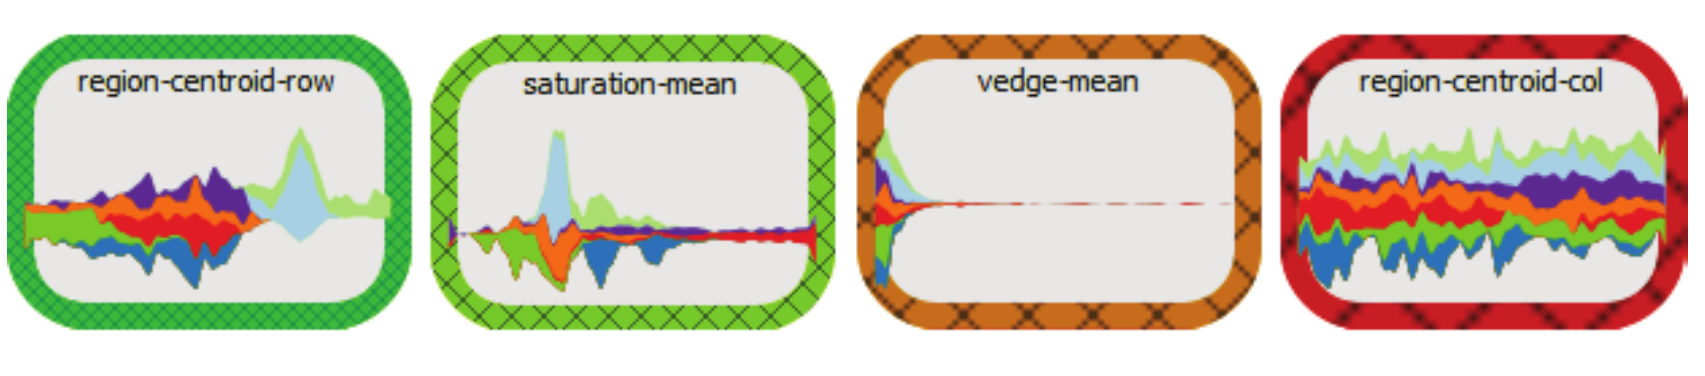
\includegraphics[width=0.8\linewidth]{images/Baobab2.png}
    \caption{The BaobabView system supports analysts with algorithmic support for selecting split attributes and presents suggestions visually. Border color indicates the goodness of the split as measured by the Gain-ratio, enabling users to make informed decisions about tree construction while maintaining control over the modeling process.}
    \label{fig:baobab_algorithmic_support}
\end{figure}

The data flow visualization capabilities of BaobabView are further illustrated in Figure \ref{fig:baobab_partitioning}, which shows how the system visualizes instance partitioning and highlights misclassifications.

% Source: TaskBased Visual Interactive Modeling Decision Trees and RuleBased Classifiers, Page: Figure 10
\begin{figure}[!htb]
    \centering
    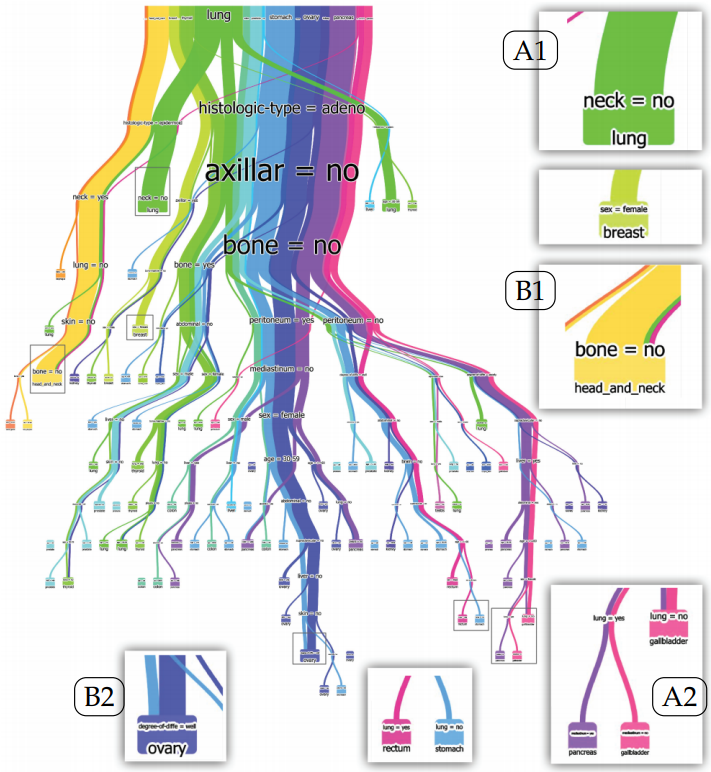
\includegraphics[width=0.8\linewidth]{images/Baobab3.png}
    \caption{BaobabView system showing the partitioning of instances.
Correct predictions are visible (A1, A2) and mis-classifications stand out
(B1, B2), enabling users to immediately identify areas where the decision tree performs poorly and may require refinement.}
    \label{fig:baobab_partitioning}
\end{figure}

\textbf{TIMBERTREK} \cite{wang2022timbertrek} introduces innovative \textbf{Sunburst diagrams} \cite{885091} for visualizing Rashomon sets of equally-performing decision trees, enabling users to explore thousands of model candidates through focus+context \cite{readingsInformationVi} interaction techniques, as demonstrated in Figure \ref{fig:timbertrek_system}.

\paragraph{Practical Tools and Libraries}

The landscape of practical implementations includes several notable tools. The \textbf{dtreeviz library} provides feature-target space visualization with \textbf{strip plots}, \textbf{scatter plots}, and decision boundary highlighting. Figure \ref{fig:tool_comparison} shows comprehensive comparisons between different tools from the library's authors' documentation on "how to visualize decision trees" \cite{parr2019dtreeviz}.

Standard machine learning libraries offer basic capabilities: \textbf{scikit-learn's plot\_tree}, \textbf{graphviz integration} for DOT format export, and \textbf{text-based representations} \cite{plonski2021visualize}. Specialized tools like the \textbf{supertree package} add interactive capabilities, including drag-and-zoom, node collapse/expand, and sample flow visualization between nodes \cite{plonski2021visualize}. Web-based implementations using \textbf{D3.js} enable interactive decision table to tree conversion and real-time traversal \cite{joesquito2024decision}.

% Source: webpage explained.ai decisiontreeviz, Multiple pages throughout document
\begin{figure}[p] 
    \centering
    \begin{subfigure}{0.5\textwidth}
        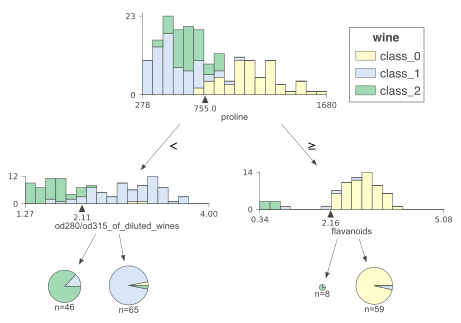
\includegraphics[width=\linewidth]{images/wine-TD-2.png}
        \caption{Wine 3-class top-down orientation}
        \label{fig:tool_comparison_wine-TD-2}
    \end{subfigure}\hfill
    \begin{subfigure}{0.5\textwidth}
        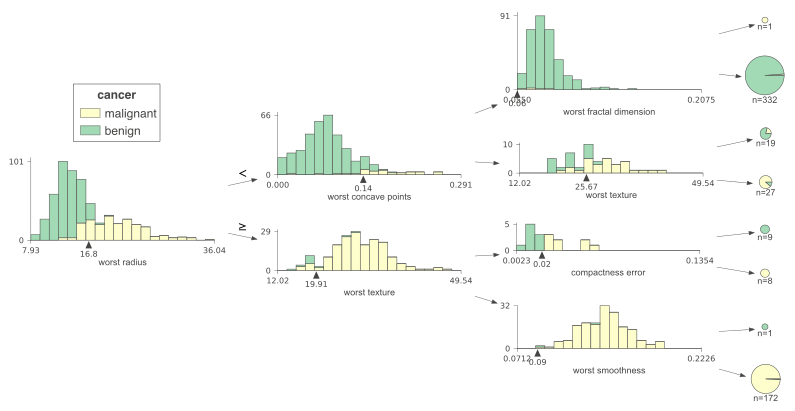
\includegraphics[width=\linewidth]{images/breast_cancer-LR-3.png}
        \caption{Breast cancer 2-class left-to-right}
        \label{fig:tool_comparison_breast_cancer-LR-3}
    \end{subfigure}
    \vspace{0.5cm} 
    \begin{subfigure}{0.48\textwidth}
        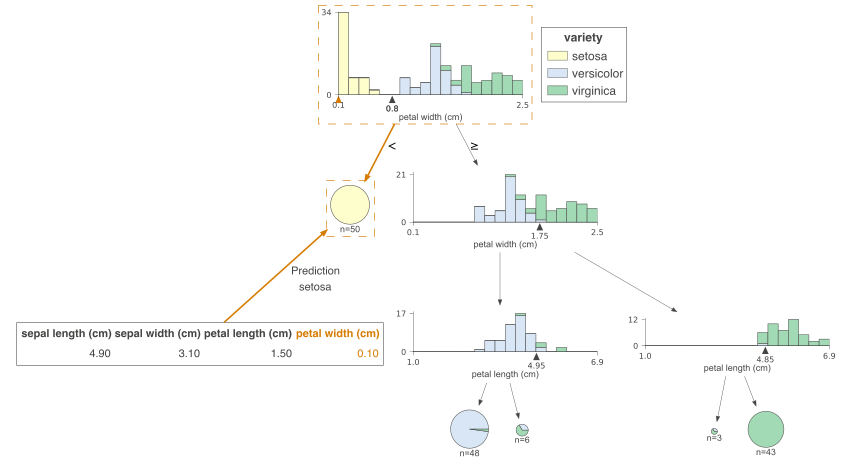
\includegraphics[width=\linewidth]{images/iris-TD-3-X.png}
        \caption{Iris 3-class showing a prediction}
        \label{fig:tool_comparison_iris-TD-3-X}
    \end{subfigure}\hfill
    \begin{subfigure}{0.48\textwidth}
        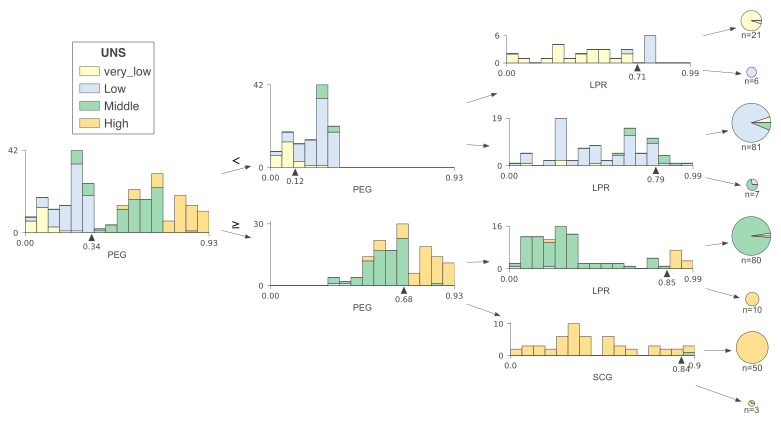
\includegraphics[width=\linewidth]{images/knowledge-LR-3.png}
        \caption{User knowledge rating 4-class}
        \label{fig:tool_comparison_knowledge-LR-3}
    \end{subfigure}
    \vspace{0.5cm}
    \begin{subfigure}{0.48\textwidth}
        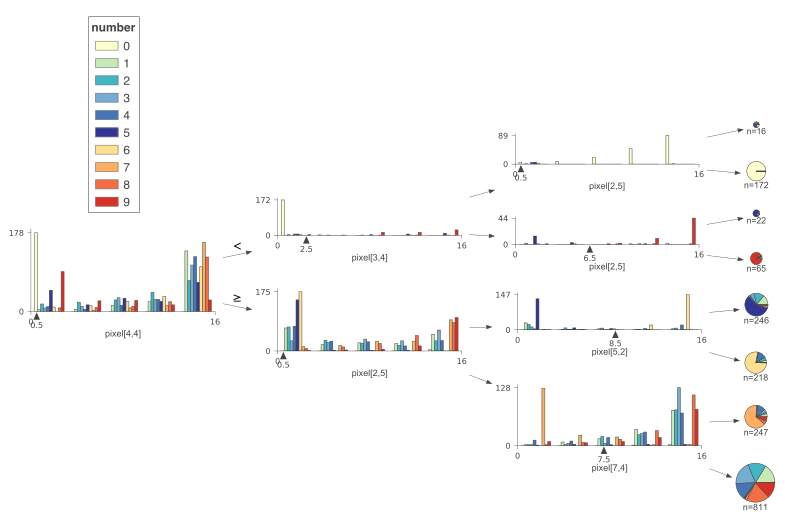
\includegraphics[width=\linewidth]{images/digits-LR-3.png}
        \caption{Digits 10-class}
        \label{fig:tool_comparison_digits-LR-3}
    \end{subfigure}\hfill
    \begin{subfigure}{0.48\textwidth}
        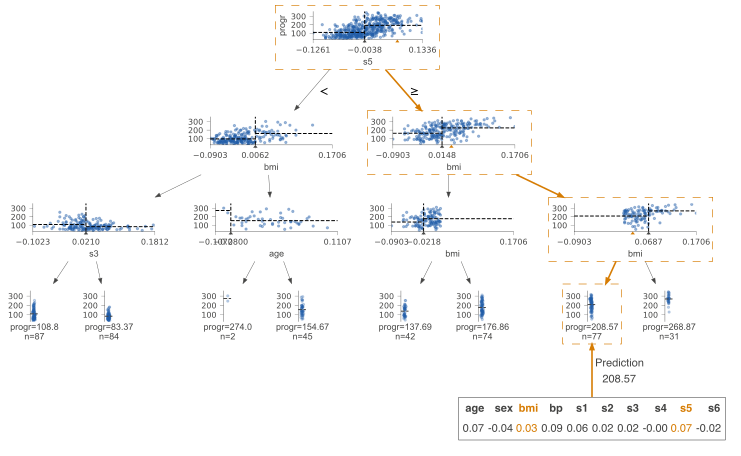
\includegraphics[width=\linewidth]{images/diabetes-TD-3-X.png}
        \caption{Diabetes showing a prediction}
        \label{fig:tool_comparison_diabetes-TD-3-X}
    \end{subfigure}
    \caption{Comprehensive comparison of decision tree visualization tools, including scikit-learn, dtreeviz, R packages, SAS, and IBM Watson. The comparison demonstrates how dtreeviz enhances traditional approaches by showing feature distributions as overlapping stacked histograms within decision nodes and using proportional leaf sizes, while maintaining clear decision boundary visualization.}
    \label{fig:tool_comparison}
\end{figure}

% Page 2 - Continuation of the same figure
\begin{figure}[p]
    \ContinuedFloat  % This keeps the same figure number
    \centering
        
    \begin{subfigure}{0.48\textwidth}
        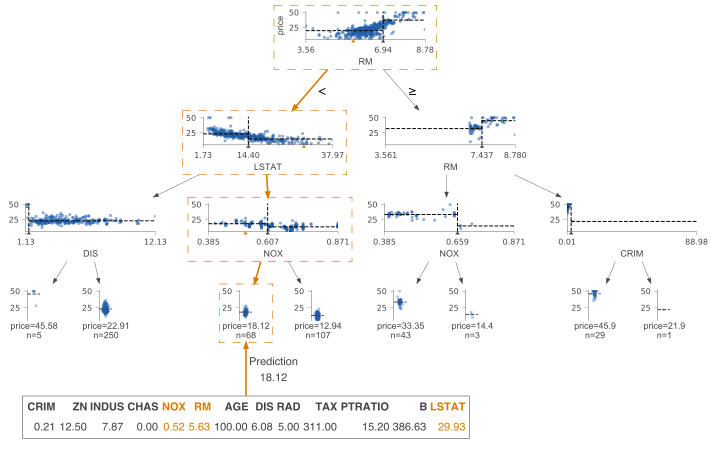
\includegraphics[width=\linewidth]{images/boston-TD-3-X.png}
        \caption{Boston showing a prediction}
        \label{fig:tool_comparison_boston-TD-3-X}
    \end{subfigure}\hfill
    \begin{subfigure}{0.48\textwidth}
        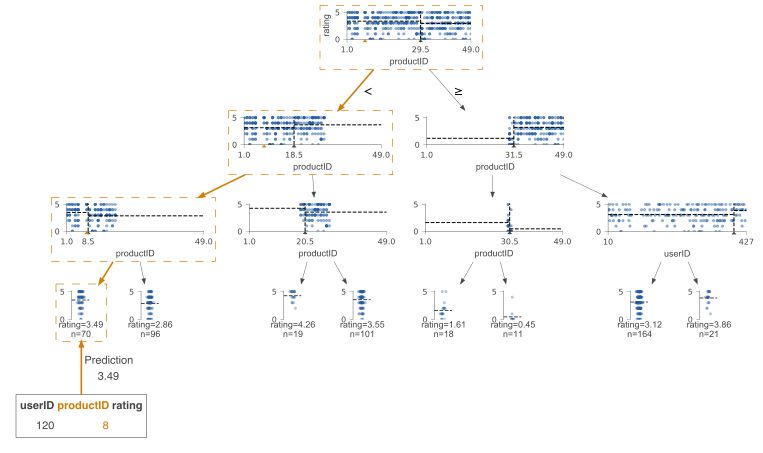
\includegraphics[width=\linewidth]{images/sweets-TD-3-X.png}
        \caption{Sweets showing a prediction}
        \label{fig:tool_comparison_sweets-TD-3-X}
    \end{subfigure}
    \vspace{0.5cm}
    
    \begin{subfigure}{0.48\textwidth}
        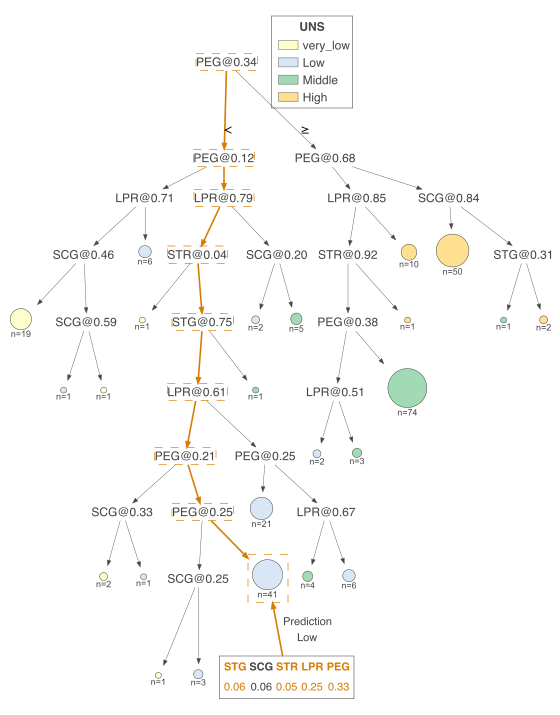
\includegraphics[width=\linewidth]{images/knowledge-TD-15-X-simple.png}
        \caption{User knowledge rating 4-class non-fancy}
        \label{fig:tool_comparison_knowledge-TD-15-X-simple}
    \end{subfigure}\hfill
    \begin{subfigure}{0.48\textwidth}
        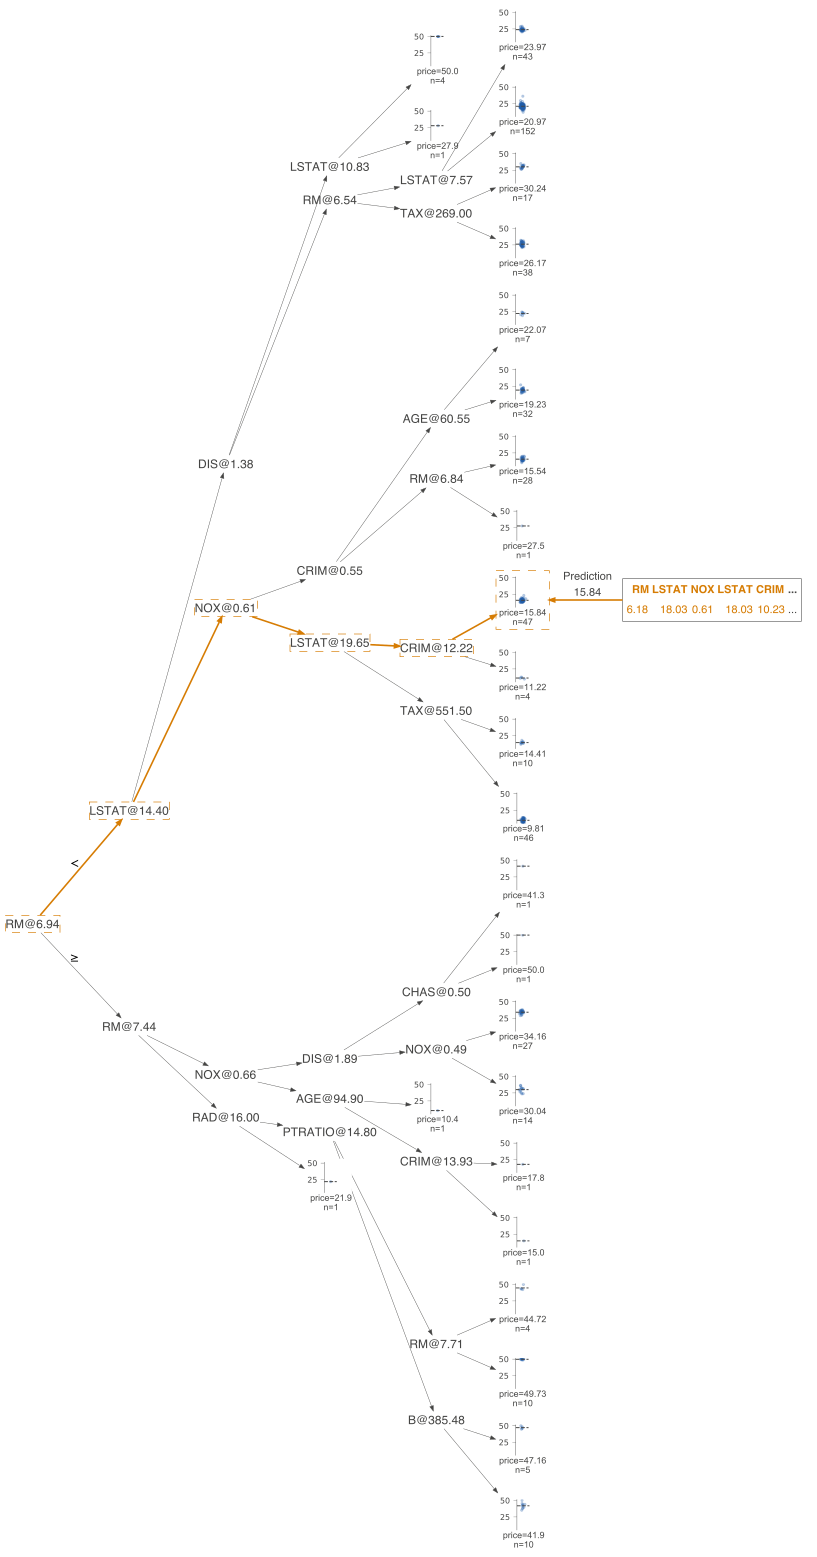
\includegraphics[width=\linewidth]{images/boston-LR-5-X-simple.png}
        \caption{Diabetes non-fancy}
        \label{fig:tool_comparison_boston-LR-5-X-simple}
    \end{subfigure}
    \caption*{Figure \ref{fig:tool_comparison} (continued)}
\end{figure}

\paragraph{Hybrid and Multi-View Approaches}

An emerging trend involves the combination of multiple visualization paradigms within unified interfaces. Van den Elzen et al. \cite{elzen2011baobabview} demonstrate the integration of tree structure visualization with data distribution views, confusion matrices, and alternative dataset exploration. Similarly, Fisher et al. \cite{fisher2012making} discuss the broader principles of coordinated multiple views, including overview and detail patterns and multiform visualizations that could be applied to decision tree contexts.

This comprehensive landscape reveals both the richness of available techniques and the fragmentation of approaches, with limited systematic evaluation of when different visualization paradigms are most effective for specific interpretability goals.

\subsubsection{Visualization Design Patterns in Decision Tree Literature}

The comprehensive analysis by Streeb et al. \cite{Streeb2021TaskBasedVI} reveals clear patterns in how decision trees are visualized across 152 publications. Their systematic categorization, presented in Tables \ref{tab:VisualDesignsOfTreesANDFurtherComponentsStreeb2021TaskBasedVI} and \ref{tab:measureStreeb2021TaskBasedVI}, demonstrates the dominance of certain approaches in current practice.

\paragraph{Visual Design Preferences}
The survey reveals a strong preference for traditional node-link diagrams, which appear in 110 of the 152 publications, making them by far the most common approach to representing tree structure. Other tree visualization techniques show much lower adoption rates: treemaps appear in only 9 publications, icicle plots in 10, and pipe diagrams in 6. This concentration suggests that despite advances in hierarchical visualization techniques, the research community largely agrees on the fact that conventional tree representations are more effective.

For additional visual components beyond the core tree structure, the analysis shows frequent use of standard statistical visualizations. Bar charts and histograms appear in more than 20 publications, line charts in almost 15, and scatter plots in more than 30. These findings indicate that researchers commonly augment tree visualizations with familiar chart types.

% % Not relevant to the current analysis
% \paragraph{Quality Measure Integration}
% Perhaps most relevant is the limited integration of quality measures in tree visualizations. Table \ref{tab:measureStreeb2021TaskBasedVI} reveals that only 79 of the 152 publications display any quality measures at all. Among those that do, accuracy dominates with more than 25 appearances, while other important measures like precision, recall, F1-score and $\chi^2$ appear in fewer than 5 publications each. This pattern suggests a significant missed opportunity for helping users understand model performance through visual means.

\paragraph{Node Design and Encoding Strategies}

% \textbf{Size Encoding for Sample Representation:} 
A consistent pattern across multiple systems involves encoding sample sizes through node dimensions. Wang et al. \cite{wang2022timbertrek} demonstrate \textbf{funnel-like node representations} where node width corresponds to the percentage of training samples, enabling users to quickly identify important decision points and assess model robustness. Similarly, Wang et al. \cite{wang2022timbertrek} employ node size variations to represent the significance of different tree components within the Rashomon set \cite{Streeb2021TaskBasedVI}.

% \textbf{Multi-layered Node Content:} 
Effective node design integrates multiple information layers without overwhelming users. Elzen et al. \cite{elzen2011baobabview} showcase nodes containing \textbf{class distributions via streamgraphs}, \textbf{attribute values}, and \textbf{split conditions}, all within compact visual representations, as demonstrated in Figure \ref{fig:baobab_interface}. Ming et al. \cite{ming2019rulematrix} demonstrate how \textbf{compact clause representations} can be combined with \textbf{data distribution previews} using histograms for continuous features and bar charts for categorical features.

% % Not relevant to the current analysis
% \textbf{Performance Indicators:} Visual encoding of prediction confidence and accuracy represents a critical best practice. Wang et al. \cite{wang2022timbertrek} use \textbf{opacity encoding for leaf node accuracy}, allowing users to quickly assess prediction confidence across the tree. Ming et al. \cite{ming2019rulematrix} integrate \textbf{evidence bars} and \textbf{fidelity metrics} directly into the node representation, providing immediate feedback on rule quality.

\paragraph{Color Coding Strategies and Accessibility}

% \textbf{Class-Based Color Schemes:} 
Consistent color coding for target classes emerges as a fundamental pattern. Parr et al. \cite{parr2019dtreeviz} emphasize the use of \textbf{handpicked colorblind-safe palettes}, with distinct schemes for different numbers of target categories (2 through 10). This approach ensures accessibility while maintaining visual coherence across complex trees.

% \textbf{Attribute and Feature Highlighting:} 
Several systems employ color to highlight important features and decision paths. Elzen et al. \cite{elzen2011baobabview} use \textbf{attribute-based node coloring} to reveal which features are most frequently used in splitting decisions. Parr et al. \cite{parr2019dtreeviz} use \textbf{orange wedge highlighting} for decision paths, making the comparison operations easily visible during tree traversal.

% \textbf{Gradient and Transparency Techniques:} 
Advanced color strategies include the use of transparency and gradients to convey additional information layers. Ming et al. \cite{ming2019rulematrix} employ \textbf{higher opacity for satisfied conditions} and \textbf{gradient coloring for confidence intervals}. Mrva et al. \cite{mrva2019decision} use \textbf{transparent rendering for filtered nodes}, allowing users to focus on specific classes while maintaining context.

\paragraph{Edge Representation and Data Flow Visualization}

% \textbf{Variable Width Edges:} 
A recurring best practice involves encoding data flow through edge thickness. Elzen et al. \cite{elzen2011baobabview} pioneer the use of \textbf{color-banded edges with variable width} to visualize the volume of data flowing through each decision branch. This technique provides immediate visual feedback about data distribution across the tree structure, as demonstrated in Figure \ref{fig:baobab_partitioning}.

% \textbf{Decision Path Highlighting:}
Multiple systems implement strategies for highlighting active decision paths. Parr et al. \cite{parr2019dtreeviz} use \textbf{thicker, colored edges} for paths involved in specific predictions, while Joesquito \cite{joesquito2024decision} employs \textbf{animated traversal} with color transitions to show decision progression in real-time.

% \textbf{Label Positioning and Clarity:} 
Consistent edge labeling practices include positioning Y/N or condition labels at strategic points along edges. Joesquito \cite{joesquito2024decision} demonstrates optimal \textbf{midpoint label placement} with appropriate spacing from both source and target nodes.

\paragraph{Layout and Spatial Organization}

% \textbf{Hierarchical Consistency:} 
Maintaining consistent spatial relationships across tree levels represents a fundamental design principle. Schulz et al. \cite{schulz2011treevis} identify \textbf{layer-based organization} as essential for preserving tree topology understanding. Elzen et al. \cite{elzen2011baobabview} implement \textbf{weighted edge algorithms} that optimize readability while minimizing edge crossings.

% \textbf{Adaptive Layouts:} 
Advanced systems implement layout algorithms that adapt to tree characteristics. Wang et al. \cite{wang2022timbertrek} introduce \textbf{focus+context techniques} \cite{readingsInformationVi} using Sunburst diagrams \cite{885091} that allow seamless transitions between overview and detail levels.

\paragraph{Integration of Data Distributions}

% \textbf{Feature-Target Space Visualization:} 
One of the best practices found involves directly integrating data distribution information within tree visualizations. Parr et al. \cite{parr2019dtreeviz} demonstrate the effectiveness of \textbf{strip plots and scatter plots} embedded within decision nodes, showing actual data distributions for split conditions, as illustrated in Figure \ref{fig:tool_comparison}. This approach eliminates the cognitive burden of connecting abstract tree structure with the underlying data patterns.

% \textbf{Contextual Distribution Views:} 
Ming et al. \cite{ming2019rulematrix} implements \textbf{conditional distribution visualization} that shows feature distributions given that previous rules are not satisfied, providing crucial context for understanding rule interactions. Mrva et al. \cite{mrva2019decision} extend this concept with \textbf{3D histograms} comparing parent and child node distributions, as shown in Figure \ref{fig:3d_medical_trees}.

\paragraph{Interaction Design Patterns}

% \textbf{Progressive Disclosure:} 
Effective interaction design balances information density with usability through progressive disclosure mechanisms. Ming et al. \cite{ming2019rulematrix} implement \textbf{details-on-demand} through hover interactions and expandable cells, while Wang et al. \cite{wang2022timbertrek} provide \textbf{repositionable tree windows} for comparative analysis, as demonstrated in Figure \ref{fig:timbertrek_system}.

% \textbf{Dynamic Filtering and Exploration:} 
Multiple systems implement sophisticated filtering capabilities. Ming et al. \cite{ming2019rulematrix} provide \textbf{rule filtering by support and confidence}, while Mrva et al. \cite{mrva2019decision} enable \textbf{class-based filtering} with transparency adjustments. Elzen et al. \cite{elzen2011baobabview} demonstrate \textbf{real-time threshold modification} with immediate visual feedback, as shown in Figure \ref{fig:baobab_algorithmic_support}.

% \textbf{Coordinated Multiple Views:} 
Advanced systems integrate tree visualization with complementary views. Elzen et al. \cite{elzen2011baobabview, 10.5555/383784} coordinate tree views with \textbf{confusion matrices}, \textbf{attribute distributions}, and \textbf{alternative dataset views}, as demonstrated in Figure \ref{fig:baobab_interface}. Fisher et al. \cite{fisher2012making} establish theoretical foundations for such coordination through \textbf{brushing and linking} techniques.

\paragraph{Typography and Readability}

% \textbf{Readable Text Design:} 
Subtle but important patterns emerge in text presentation. Parr et al. \cite{parr2019dtreeviz} advocate for \textbf{gray rather than black text} to reduce eye strain, while maintaining sufficient contrast for accessibility. \textbf{Hairline borders} and \textbf{outlined shapes} improve element separation without overwhelming visual complexity.

% \textbf{Hierarchical Information Architecture:} 
Effective systems organize textual information hierarchically within nodes. Ming et al. \cite{ming2019rulematrix} demonstrate \textbf{matrix organization} where feature order remains consistent across rules, facilitating rapid visual comparison and rule understanding, as illustrated in Figure \ref{fig:rulematrix_pipeline}.

These patterns collectively establish a foundation for effective surrogate models visualization, emphasizing the importance of integrating multiple information dimensions while maintaining visual clarity and supporting diverse interaction paradigms. 
The latter analysis of various pieces of literature provides a comprehensive framework for future decision tree visualization development, highlighting both well-established practices and emerging innovative approaches that push the boundaries of traditional tree representation techniques.
